%!TEX program = xelatex
\documentclass[aspectratio=169,11pt]{ctexbeamer}

\usepackage[bluetheme]{ustcbeamer}
\input{ustctheme.tex}

\usepackage{booktabs}
\usepackage{tabularx}
\usepackage{array}
\usepackage{graphicx}
\usepackage{tikz}
\usepackage{fontspec}
\usetikzlibrary{arrows.meta,positioning,shapes.geometric}

\graphicspath{{figures/final_defense/}{figures/project/}{figures/}}

\IfFontExistsTF{Arial}{\setmainfont{Arial}}{}
\IfFontExistsTF{PingFang SC}{\setCJKmainfont{PingFang SC}}{}

\setbeamertemplate{navigation symbols}{}
\setbeamerfont{frametitle}{size=\large,series=\bfseries}
\setbeamertemplate{frametitle}{%
  \nointerlineskip
  \vskip0.45ex
  \begin{beamercolorbox}[wd=.68\paperwidth,ht=2.2ex,dp=0.7ex,leftskip=0.75em]{frametitle}
    \usebeamerfont{frametitle}\insertframetitle
  \end{beamercolorbox}
}
\setbeamerfont{normal text}{size=\normalsize}
\setlength{\parskip}{0.22em}

\definecolor{phmblue}{RGB}{0,64,152}
\definecolor{phmlight}{RGB}{239,246,255}
\definecolor{phmline}{RGB}{180,202,232}
\definecolor{phmgreen}{RGB}{29,128,99}
\definecolor{phmorange}{RGB}{214,116,32}
\definecolor{phmgray}{RGB}{75,85,99}
\definecolor{phmred}{RGB}{190,50,45}

\newcolumntype{Y}{>{\raggedright\arraybackslash}X}
\newcolumntype{C}{>{\centering\arraybackslash}X}

\newcommand{\takeaway}[1]{%
  \vspace{0.18em}
  \begin{beamercolorbox}[wd=\linewidth,rounded=true,sep=0.58em]{block body}
    \parbox{\dimexpr\linewidth-1.16em\relax}{\raggedright\small\color{phmblue}\bfseries #1}
  \end{beamercolorbox}
}

\newcommand{\metricbox}[3]{%
  \begin{beamercolorbox}[wd=#1,rounded=true,sep=0.48em,center]{block body}
    {\Large\bfseries\color{phmblue}#2}\par
    {\scriptsize\color{phmgray}#3}
  \end{beamercolorbox}
}

\newcommand{\smallcap}[1]{%
  {\scriptsize\color{phmgray}#1}
}

\newcommand{\linkline}[2]{%
  {\scriptsize\color{phmblue}\href{#1}{#2}}
}

\newcommand{\code}[1]{\texttt{#1}}

\title[轴承 PHM 结题答辩]{轴承预测性维护中的剩余寿命预测与故障分析}
\subtitle{}
\author[周逸进]{汇报人：周逸进 \quad 小组成员：周逸进、朱德豪、蔡祎珏、邹扬}
\institute[USTC]{中国科学技术大学 \quad 软件学院}
\date{2026 年 6 月}

\begin{document}

\maketitleframe

\section{研究背景}

\begin{frame}[t]{研究背景：从故障诊断走向预测性维护}
  \begin{columns}[T,onlytextwidth]
    \begin{column}{0.32\textwidth}
      \begin{block}{轴承为什么重要}
        \begin{itemize}
          \item 旋转机械中的关键支撑部件
          \item 退化会引起振动、噪声和精度下降
          \item 严重时造成停机和连锁损伤
        \end{itemize}
      \end{block}
    \end{column}
    \begin{column}{0.32\textwidth}
      \begin{block}{只做故障分类不够}
        \begin{itemize}
          \item 分类回答“是否异常”
          \item 工程上还要知道“还能用多久”
          \item 需要更早的退化预警
        \end{itemize}
      \end{block}
    \end{column}
    \begin{column}{0.32\textwidth}
      \begin{block}{本文目标}
        \begin{itemize}
          \item 建立三任务 PHM 实验闭环
          \item 解释特征为什么有效
          \item 输出可复查的训练与展示材料
        \end{itemize}
      \end{block}
    \end{column}
  \end{columns}

  \vspace{1.0em}
  \centering
  \resizebox{0.94\linewidth}{!}{%
  \begin{tikzpicture}[x=1cm,y=1cm]
    \node[draw=phmline, fill=phmlight, rounded corners, minimum width=2.9cm, minimum height=0.72cm] (a) at (0,0) {振动信号};
    \node[draw=phmline, fill=phmlight, rounded corners, minimum width=2.9cm, minimum height=0.72cm] (b) at (3.8,0) {特征分析};
    \node[draw=phmblue, fill=phmblue!8, rounded corners, very thick, minimum width=3.1cm, minimum height=0.72cm] (c) at (7.7,0) {三任务建模};
    \node[draw=phmgreen, fill=phmgreen!8, rounded corners, very thick, minimum width=3.1cm, minimum height=0.72cm] (d) at (11.6,0) {训练演示};
    \draw[->, very thick, phmblue] (a) -- (b);
    \draw[->, very thick, phmblue] (b) -- (c);
    \draw[->, very thick, phmblue] (c) -- (d);
  \end{tikzpicture}
  }
\end{frame}

\begin{frame}[t]{任务定义：预测、识别与预警}
  \begin{table}
    \scriptsize
    \begin{tabularx}{\linewidth}{lcllY}
      \toprule
      任务 & 类型 & 输出 & 指标 & 工程作用 \\
      \midrule
      RUL & 回归 & \code{linear\_rul\_norm} & RMSE & 预测当前样本距离寿命终点的归一化剩余比例。 \\
      HealthState & 四分类 & \code{health\_state\_id} & WeightedF1 & 识别健康、轻微退化、中度退化和严重退化阶段。 \\
      EarlyFault & 二分类 & \code{early\_fault} & WeightedF1 & 判断是否进入早期异常或早期故障预警阶段。 \\
      \bottomrule
    \end{tabularx}
  \end{table}

  \vspace{0.5em}
  \begin{columns}[T,onlytextwidth]
    \begin{column}{0.49\textwidth}
      \begin{block}{标签说明}
        \begin{itemize}
          \item RUL 采用 \code{linear\_rul\_norm} 表示剩余寿命比例
          \item HealthState 描述轴承退化阶段
          \item EarlyFault 描述是否进入早期预警状态
        \end{itemize}
      \end{block}
    \end{column}
    \begin{column}{0.49\textwidth}
      \begin{block}{实验设计}
        \begin{itemize}
          \item 使用 GRU 序列模型学习连续退化过程
          \item 用现场命令展示数据到任务样本的链路
          \item 复现实验用于参照典型论文方法
        \end{itemize}
      \end{block}
    \end{column}
  \end{columns}

  \takeaway{三个任务分别覆盖“还能运行多久”“当前退化到哪里”“是否需要早期预警”。}
\end{frame}

\begin{frame}[t]{标签构造：RUL 与 HI/FPT}
  \begin{columns}[T,onlytextwidth]
    \begin{column}{0.32\textwidth}
      \begin{block}{RUL 标签}
        \begin{itemize}
          \item 按单个轴承内部时间顺序构造
          \item 寿命早期接近 1
          \item 寿命终点接近 0
          \item 使用 \code{linear\_rul\_norm}
        \end{itemize}
      \end{block}
    \end{column}
    \begin{column}{0.32\textwidth}
      \begin{block}{FPT 定位}
        \begin{itemize}
          \item 以 RMS 类特征构造健康指标 HI
          \item 前 20\% 样本作为健康基准段
          \item 采用 3-sigma 阈值法
          \item 阈值：$\mu_{\mathrm{base}} + 3\sigma_{\mathrm{base}}$
          \item 连续 3 个点超过阈值记为 FPT
        \end{itemize}
      \end{block}
    \end{column}
    \begin{column}{0.32\textwidth}
      \begin{block}{分类标签}
        \begin{itemize}
          \item EarlyFault：FPT 前为 0，FPT 后为 1
          \item HealthState：FPT 前为 healthy
          \item FPT 后按退化进度切为 slight / moderate / severe
          \item 分类标签均解释为退化伪标签
        \end{itemize}
      \end{block}
    \end{column}
  \end{columns}

  \vspace{0.3em}
  \centering
  \small
  \[
    \mathrm{linear\_rul\_norm}(t)=1-\frac{t}{T-1}
  \]

\end{frame}

\section{数据与特征}

\begin{frame}[t]{数据集与划分原则}
  \begin{columns}[T,onlytextwidth]
    \begin{column}{0.49\textwidth}
      \begin{block}{XJTU-SY}
        \begin{itemize}
          \item 多工况全寿命轴承振动数据
          \item 3 个工况，每个工况 5 个轴承
          \item 用于检验跨轴承和多工况泛化
        \end{itemize}
      \end{block}
      \centering
      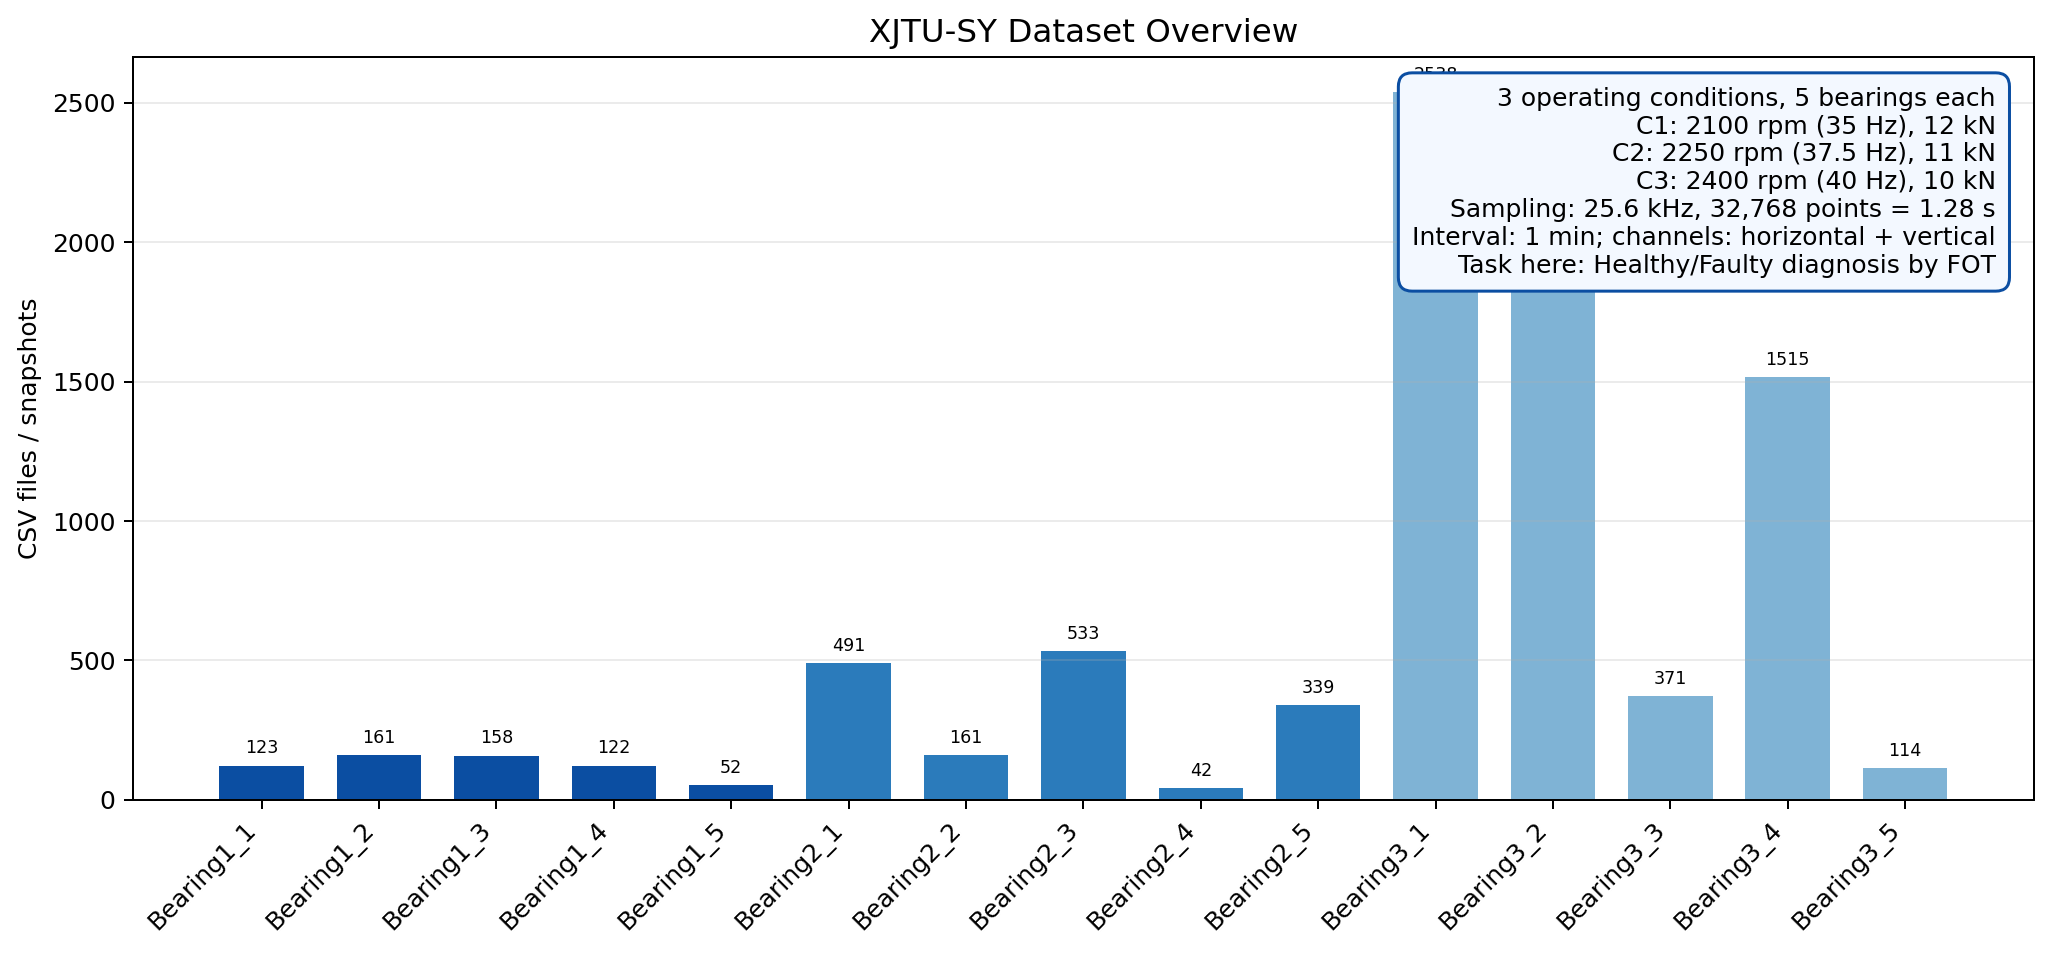
\includegraphics[width=\linewidth,height=0.33\textheight,keepaspectratio]{xjtu_dataset_overview.png}
    \end{column}
    \begin{column}{0.49\textwidth}
      \begin{block}{PHM2012}
        \begin{itemize}
          \item 轴承预测挑战数据集
          \item 包含学习集和测试集语义
          \item 用于经典 RUL 预测场景验证
        \end{itemize}
      \end{block}
      \centering
      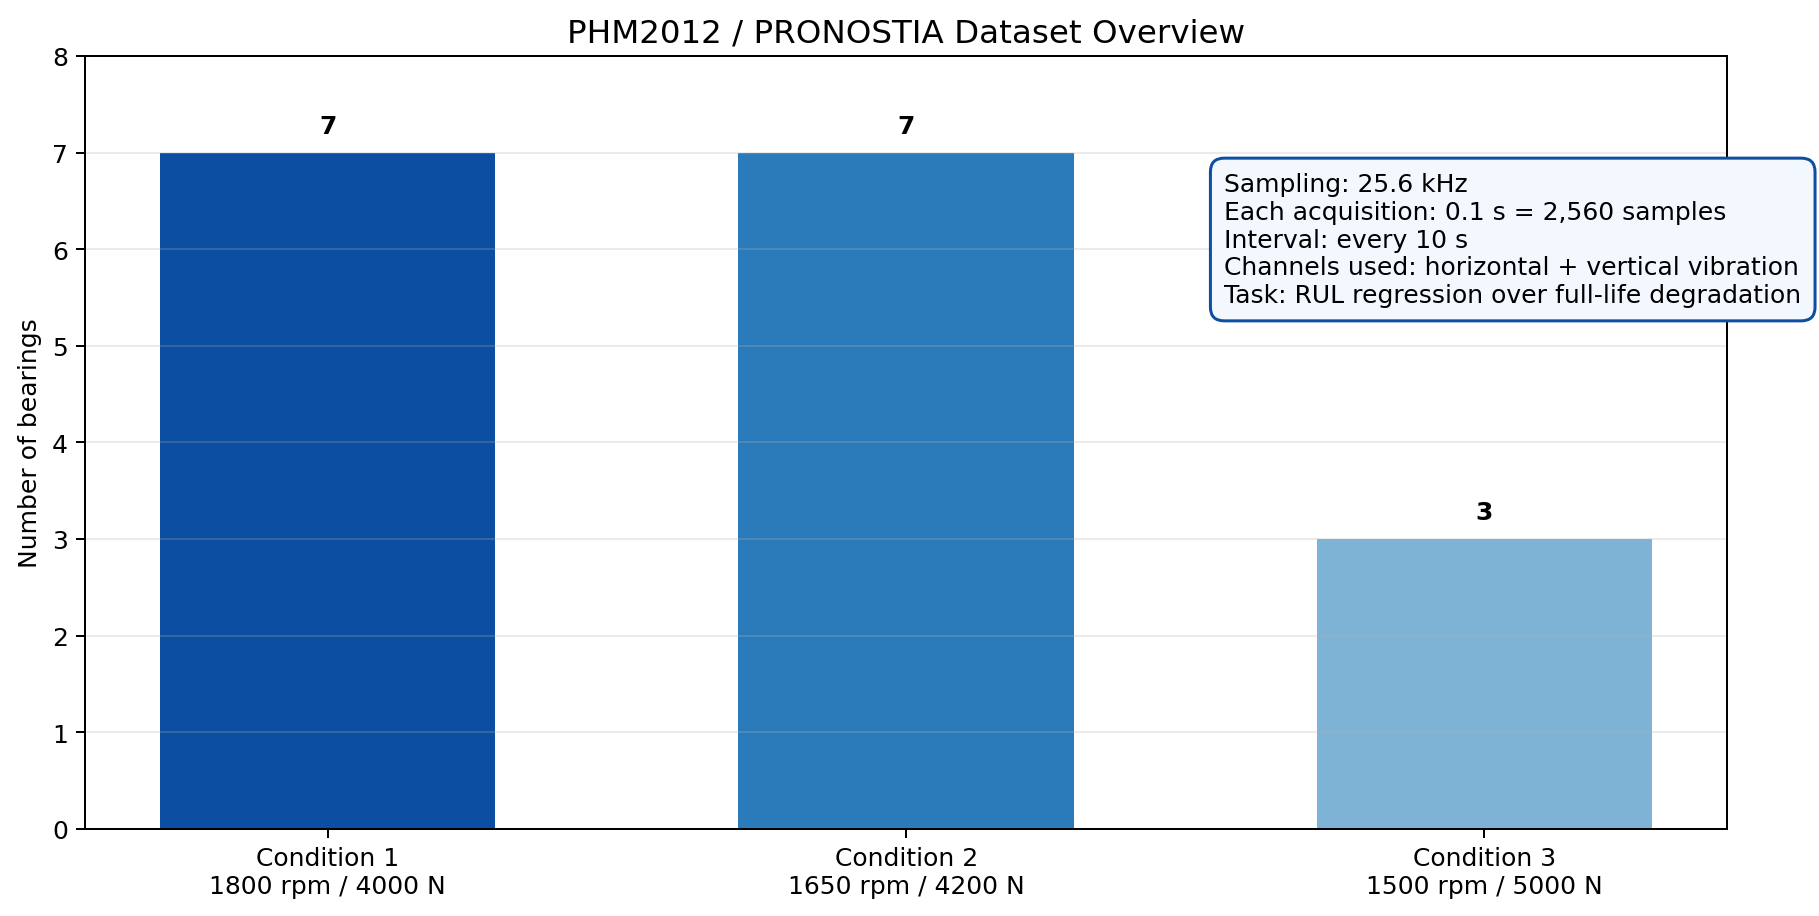
\includegraphics[width=\linewidth,height=0.33\textheight,keepaspectratio]{phm2012_dataset_overview.png}
    \end{column}
  \end{columns}

  \takeaway{按轴承或官方语义划分数据；序列样本不跨轴承、不跨数据子集。}
\end{frame}

\begin{frame}[t]{数据处理流程}
  \centering
  \resizebox{0.96\linewidth}{!}{%
  \begin{tikzpicture}[
    node distance=0.55cm,
    box/.style={rectangle, rounded corners, draw=phmblue!70, fill=phmblue!6, thick, align=center, minimum width=2.2cm, minimum height=0.7cm},
    arr/.style={-{Latex[length=2mm]}, thick, phmblue}
  ]
    \node[box] (raw) {原始振动\\信号};
    \node[box, right=of raw] (snap) {振动快照\\窗口样本};
    \node[box, right=of snap] (feat) {manual\_basic\\特征};
    \node[box, right=of feat] (clean) {train-only\\清洗标准化};
    \node[box, right=of clean] (label) {HI/FPT\\三任务标签};
    \node[box, right=of label] (seq) {Tabular /\\Sequence};
    \draw[arr] (raw) -- (snap);
    \draw[arr] (snap) -- (feat);
    \draw[arr] (feat) -- (clean);
    \draw[arr] (clean) -- (label);
    \draw[arr] (label) -- (seq);
  \end{tikzpicture}
  }

  \vspace{1.0em}
  \begin{columns}[T,onlytextwidth]
    \begin{column}{0.48\textwidth}
      \begin{block}{manual\_basic 特征}
        \begin{itemize}
          \item 时域：RMS、mean\_abs、std、ptp、kurtosis
          \item 频域：spectral centroid、entropy、band energy
          \item 通道：水平、垂直、合成幅值 mag
        \end{itemize}
      \end{block}
    \end{column}
    \begin{column}{0.48\textwidth}
      \begin{block}{序列建模}
        \begin{itemize}
          \item 表格模型使用单个窗口级特征
          \item GRU 使用长度 8 的连续特征序列
          \item 标准化参数只从训练集估计
        \end{itemize}
      \end{block}
    \end{column}
  \end{columns}
\end{frame}

\begin{frame}[t]{特征分析：从经验输入到任务证据}
  \begin{columns}[T,onlytextwidth]
    \begin{column}{0.49\textwidth}
      \centering
      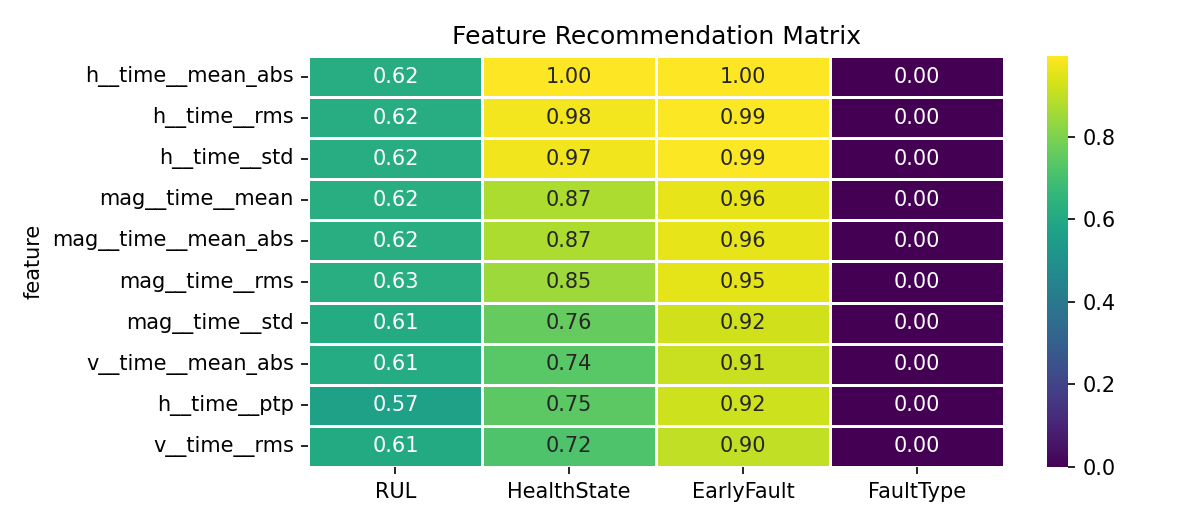
\includegraphics[width=\linewidth,height=0.55\textheight,keepaspectratio]{xjtu_feature_recommendation_matrix.png}
      \smallcap{XJTU-SY 三任务推荐特征矩阵}
    \end{column}
    \begin{column}{0.49\textwidth}
      \centering
      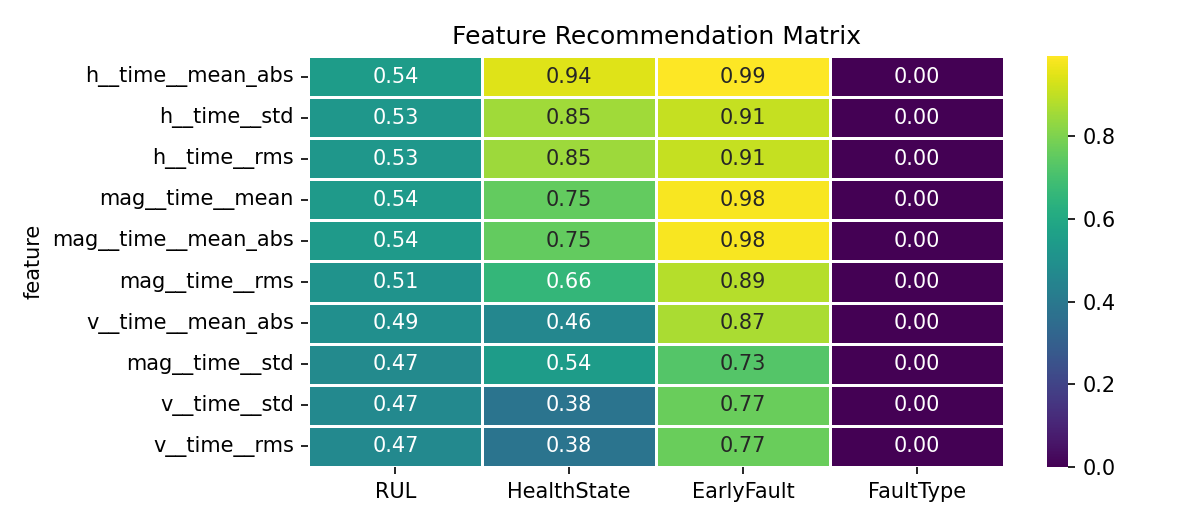
\includegraphics[width=\linewidth,height=0.55\textheight,keepaspectratio]{phm_feature_recommendation_matrix.png}
      \smallcap{PHM2012 三任务推荐特征矩阵}
    \end{column}
  \end{columns}

  \takeaway{RUL 看退化趋势；EarlyFault 看故障前后差异。}
\end{frame}

\begin{frame}[t]{特征与任务相关性如何量化}
  \begin{columns}[T,onlytextwidth]
    \begin{column}{0.32\textwidth}
      \begin{block}{RUL：退化趋势}
        \begin{itemize}
          \item Spearman：特征排序与寿命进程排序是否一致
          \item 单调性：是否随退化方向稳定升降
          \item 稳健性：是否受局部波动影响较小
        \end{itemize}
      \end{block}
    \end{column}
    \begin{column}{0.32\textwidth}
      \begin{block}{HealthState：阶段可分性}
        \begin{itemize}
          \item 互信息：特征对阶段标签的信息量
          \item Fisher score：类间差异与类内波动之比
          \item ANOVA F：不同健康阶段均值差异
        \end{itemize}
      \end{block}
    \end{column}
    \begin{column}{0.32\textwidth}
      \begin{block}{EarlyFault：故障前后差异}
        \begin{itemize}
          \item Cohen's d：正常/异常两组均值差异
          \item AUC：单个特征区分两类的能力
          \item 方向一致性：跨轴承差异方向是否稳定
        \end{itemize}
      \end{block}
    \end{column}
  \end{columns}

  \vspace{0.5em}
  \begin{beamercolorbox}[wd=\linewidth,rounded=true,sep=0.6em]{block body}
    \small
    热力图中的值是归一化后的任务适配分数，不是模型准确率，也不是原始振动幅值。
    分数越高，表示该特征越适合对应任务。
  \end{beamercolorbox}

  \takeaway{RUL 看趋势稳定性；分类任务看标签可分性。}
\end{frame}

\begin{frame}[t]{代表性特征证据}
  \begin{columns}[T,onlytextwidth]
    \begin{column}{0.50\textwidth}
      \centering
      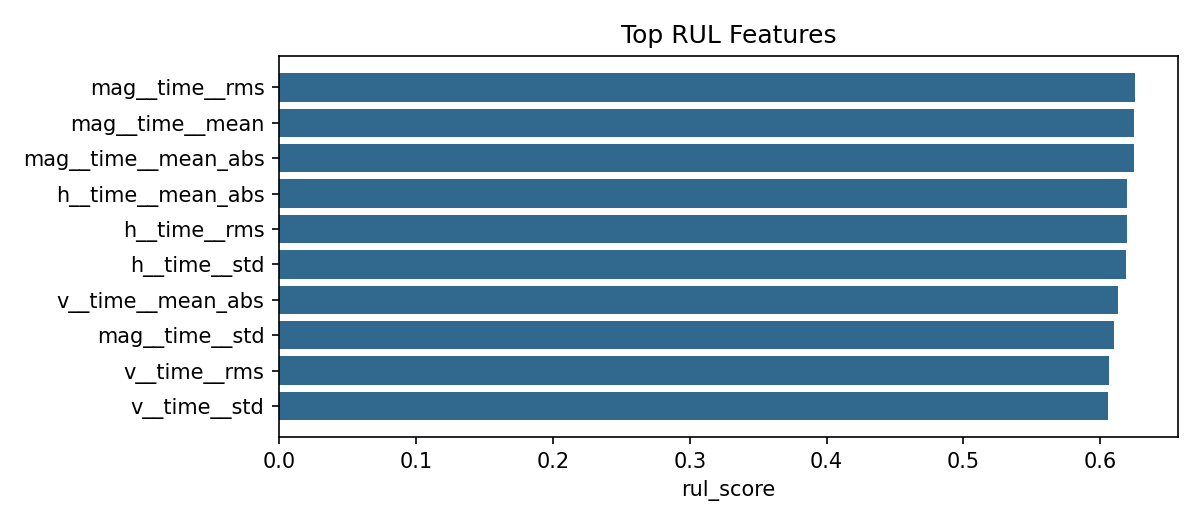
\includegraphics[width=\linewidth,height=0.58\textheight,keepaspectratio]{xjtu_rul_top_features.png}
      \smallcap{XJTU-SY RUL 相关特征排序}
    \end{column}
    \begin{column}{0.47\textwidth}
      \centering
      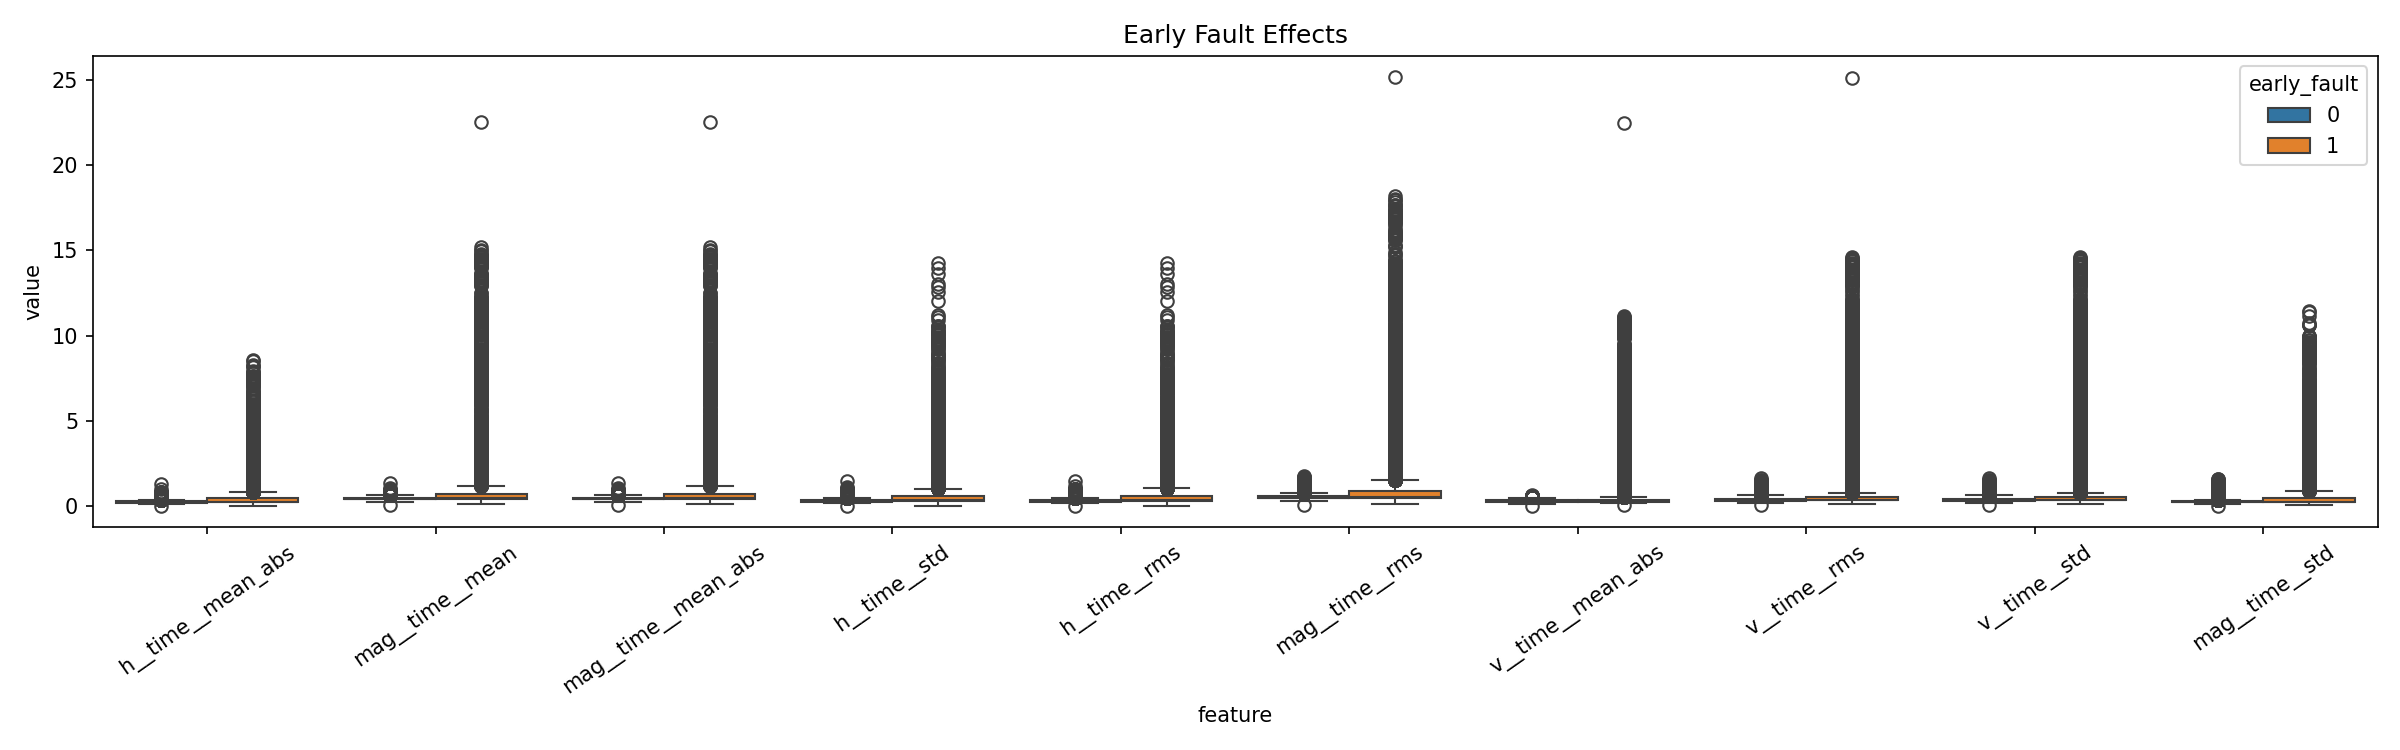
\includegraphics[width=\linewidth,height=0.58\textheight,keepaspectratio]{phm_early_fault_effects.png}
      \smallcap{PHM2012 EarlyFault 特征效应}
    \end{column}
  \end{columns}

  \takeaway{特征分析解释输入为什么适合对应任务。}
\end{frame}

\section{模型与实验}

\begin{frame}[t]{模型设计与对照结果}
  \begin{columns}[T,onlytextwidth]
    \begin{column}{0.50\textwidth}
      \begin{block}{本文方法实验}
        \begin{itemize}
          \item MLP：基础表格神经网络
          \item XGBoost / RandomForest：传统表格对照模型
          \item GRU：长度 8 的连续特征序列
        \end{itemize}
      \end{block}
      \begin{block}{EarlyFault 代表性测试结果}
        \scriptsize
        \begin{tabularx}{\linewidth}{lCC}
          \toprule
          模型 & XJTU-SY & PHM2012 \\
          \midrule
          MLP & 0.842 & 0.665 \\
          XGBoost & 0.839 & 0.578 \\
          RandomForest & 0.837 & 0.613 \\
          GRU & 0.852 & 0.683 \\
          \bottomrule
        \end{tabularx}
        \smallcap{指标为测试集 WeightedF1，数值越高越好}
      \end{block}
    \end{column}
    \begin{column}{0.46\textwidth}
      \begin{block}{任务 Head}
        \begin{itemize}
          \item RUL：1 维回归输出
          \item HealthState：4 类 logits
          \item EarlyFault：2 类 logits
        \end{itemize}
      \end{block}
      \begin{block}{论文复现实验}
        \begin{itemize}
          \item CAM-LSTM 复现模型：PHM2012 RUL
          \item 故障诊断复现模型：XJTU-SY 二分类
          \item 不参与 HealthState 四分类结论
        \end{itemize}
      \end{block}
    \end{column}
  \end{columns}

  \takeaway{EarlyFault 上 GRU 与强表格模型接近或更优；RUL 结合曲线谨慎解释。}
\end{frame}

\begin{frame}[t]{GRU 序列模型架构}
  \centering
  \resizebox{0.96\linewidth}{!}{%
  \begin{tikzpicture}[
    node distance=1.2cm,
    box/.style={draw=phmblue, rounded corners, thick, fill=phmlight, align=center, minimum width=2.5cm, minimum height=0.95cm},
    head/.style={draw=phmgreen, rounded corners, thick, fill=green!8, align=center, minimum width=2.45cm, minimum height=0.9cm},
    arr/.style={-{Latex[length=3mm]}, thick, color=phmblue}
  ]
    \node[box] (seq) {长度 8 的\\feature sequence};
    \node[box, right=of seq] (gru) {GRU 编码器\\按时间步更新 hidden state};
    \node[box, right=of gru] (last) {最后时刻\\hidden state};
    \node[head, above right=0.55cm and 1.1cm of last] (rul) {RUL Head\\1 维回归};
    \node[head, right=1.1cm of last] (health) {HealthState Head\\4 类 logits};
    \node[head, below right=0.55cm and 1.1cm of last] (early) {EarlyFault Head\\2 类 logits};
    \draw[arr] (seq) -- (gru);
    \draw[arr] (gru) -- (last);
    \draw[arr] (last) -- (rul);
    \draw[arr] (last) -- (health);
    \draw[arr] (last) -- (early);
  \end{tikzpicture}
  }

  \vspace{0.45em}
  \begin{columns}[T,onlytextwidth]
    \begin{column}{0.48\textwidth}
      \begin{block}{输入}
        \begin{itemize}
          \item 每个时间步是一行 manual\_basic 特征
          \item 序列长度为 8，不跨轴承、不跨 split
        \end{itemize}
      \end{block}
    \end{column}
    \begin{column}{0.48\textwidth}
      \begin{block}{输出}
        \begin{itemize}
          \item RUL 使用回归损失
          \item HealthState / EarlyFault 使用分类损失
        \end{itemize}
      \end{block}
    \end{column}
  \end{columns}

  \takeaway{GRU 利用连续窗口的时间顺序，而不是只看单个窗口。}
\end{frame}

\begin{frame}[t]{论文复现模型架构}
  \begin{columns}[T,onlytextwidth]
    \begin{column}{0.48\textwidth}
      \begin{block}{PHM2012 RUL 复现}
        \begin{itemize}
          \item CBAM-CNN-LSTM / CAM-LSTM 思路
          \item 用于剩余寿命曲线预测
        \end{itemize}
      \end{block}
      \centering
      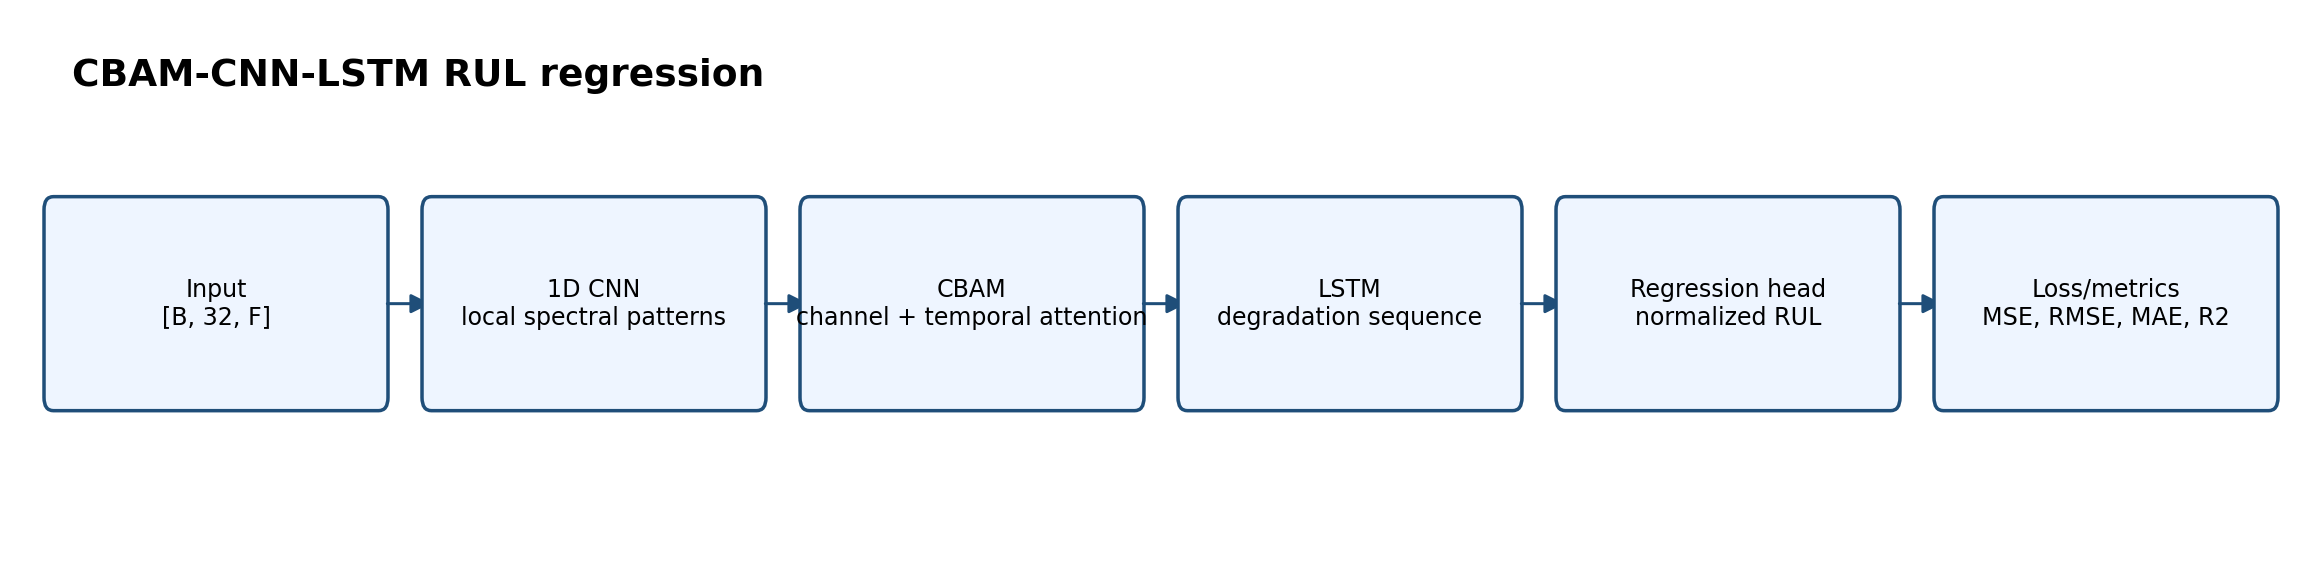
\includegraphics[width=\linewidth,height=0.38\textheight,keepaspectratio]{repro_rul_model_architecture.png}
    \end{column}
    \begin{column}{0.48\textwidth}
      \begin{block}{XJTU-SY 故障诊断复现}
        \begin{itemize}
          \item 深度故障诊断模型
          \item 用于二分类故障诊断对照
        \end{itemize}
      \end{block}
      \centering
      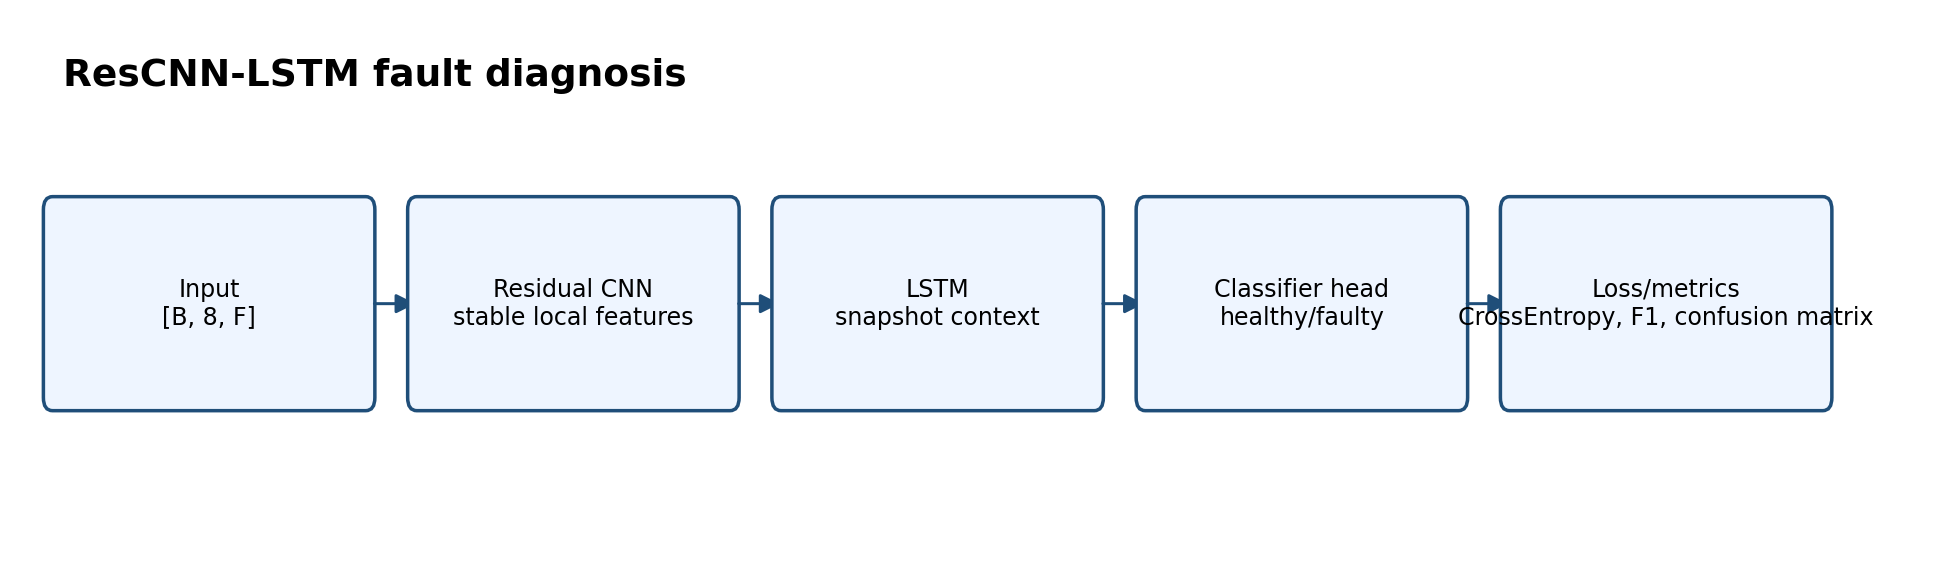
\includegraphics[width=\linewidth,height=0.38\textheight,keepaspectratio]{repro_fault_model_architecture.png}
    \end{column}
  \end{columns}

  \takeaway{复现实验是独立对照，不替代本文三任务 GRU 框架。}
\end{frame}

\begin{frame}[t]{GRU 序列模型实验结果}
  \begin{table}
    \scriptsize
    \begin{tabularx}{\linewidth}{llccY}
      \toprule
      数据集 & 任务 & 指标 & 测试集结果 & 解读 \\
      \midrule
      XJTU-SY & RUL & RMSE & 0.275009 & 能形成连续寿命趋势，但跨轴承泛化仍需谨慎。 \\
      XJTU-SY & HealthState & WeightedF1 & 0.375525 & 四阶段伪标签任务较难。 \\
      XJTU-SY & EarlyFault & WeightedF1 & 0.851679 & 当前最稳定的正向分类结果。 \\
      PHM2012 & RUL & RMSE & 0.280362 & 官方语义划分下可展示寿命趋势。 \\
      PHM2012 & HealthState & WeightedF1 & 0.417599 & 阶段识别仍有提升空间。 \\
      PHM2012 & EarlyFault & WeightedF1 & 0.682715 & 有预警能力，但弱于 XJTU-SY。 \\
      \bottomrule
    \end{tabularx}
  \end{table}

  \takeaway{EarlyFault 最稳定；RUL 保守解释；HealthState 难度最高。}
\end{frame}

\begin{frame}[t]{RUL 结果图：趋势可见，泛化仍难}
  \begin{columns}[T,onlytextwidth]
    \begin{column}{0.55\textwidth}
      \centering
      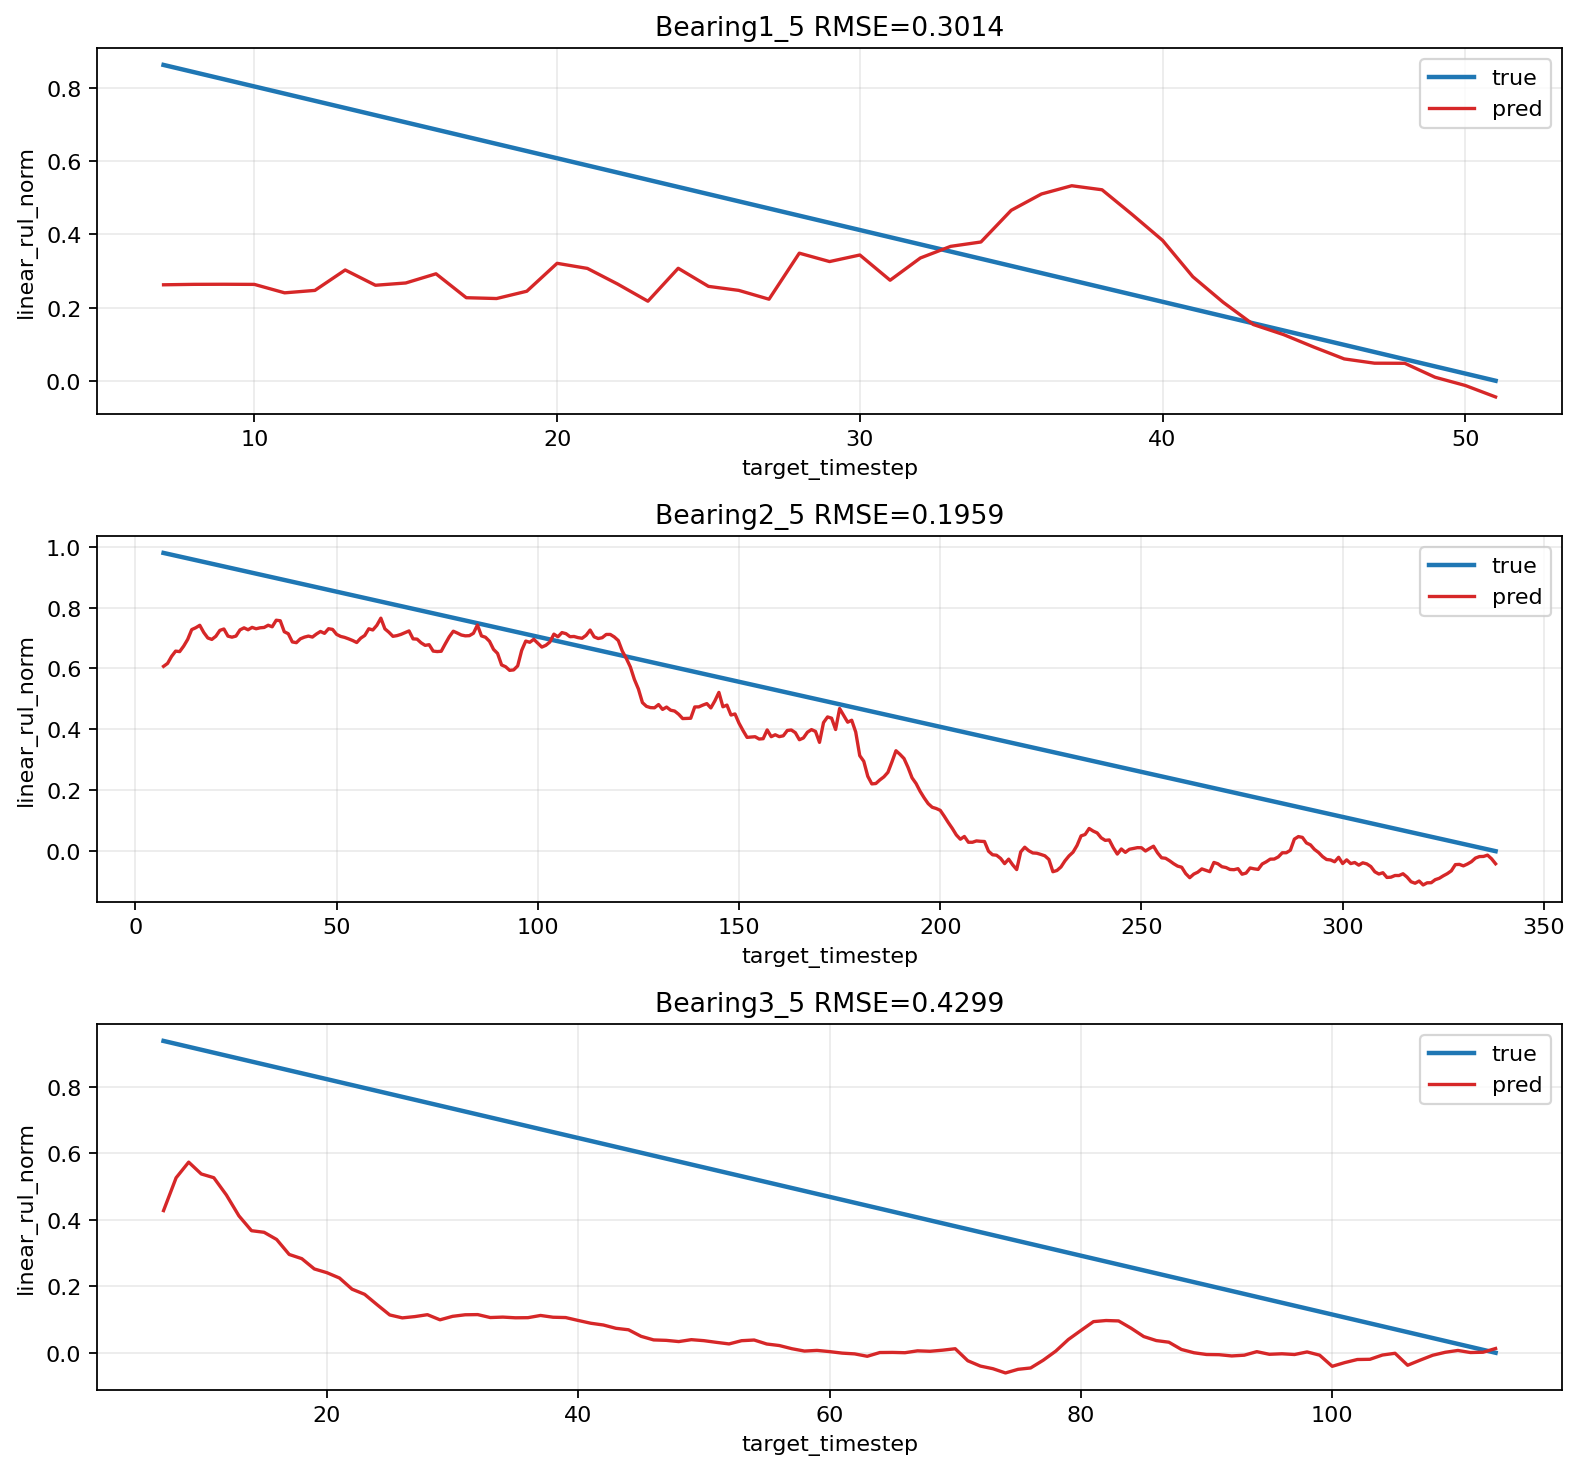
\includegraphics[width=\linewidth,height=0.61\textheight,keepaspectratio]{xjtu_gru_rul_true_pred_by_bearing.png}
      \smallcap{XJTU-SY GRU RUL 分轴承预测曲线}
    \end{column}
    \begin{column}{0.42\textwidth}
      \centering
      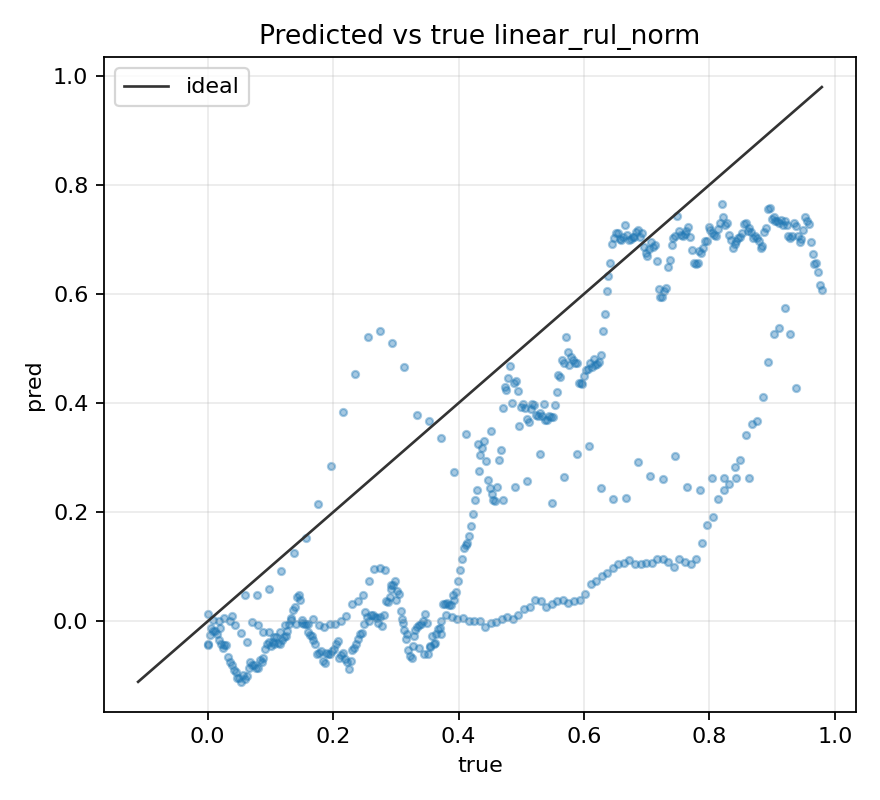
\includegraphics[width=\linewidth,height=0.38\textheight,keepaspectratio]{xjtu_gru_rul_pred_vs_true.png}
      \smallcap{预测值与真实值散点图}
      \vspace{0.4em}
      \begin{block}{读图口径}
        \begin{itemize}
          \item RUL 使用 \code{linear\_rul\_norm}
          \item 图中能看到整体寿命下降趋势
          \item 不同轴承误差仍明显，不能夸大精度
        \end{itemize}
      \end{block}
    \end{column}
  \end{columns}
\end{frame}

\begin{frame}[t]{EarlyFault 结果图：当前最稳的分类任务}
  \begin{columns}[T,onlytextwidth]
    \begin{column}{0.48\textwidth}
      \centering
      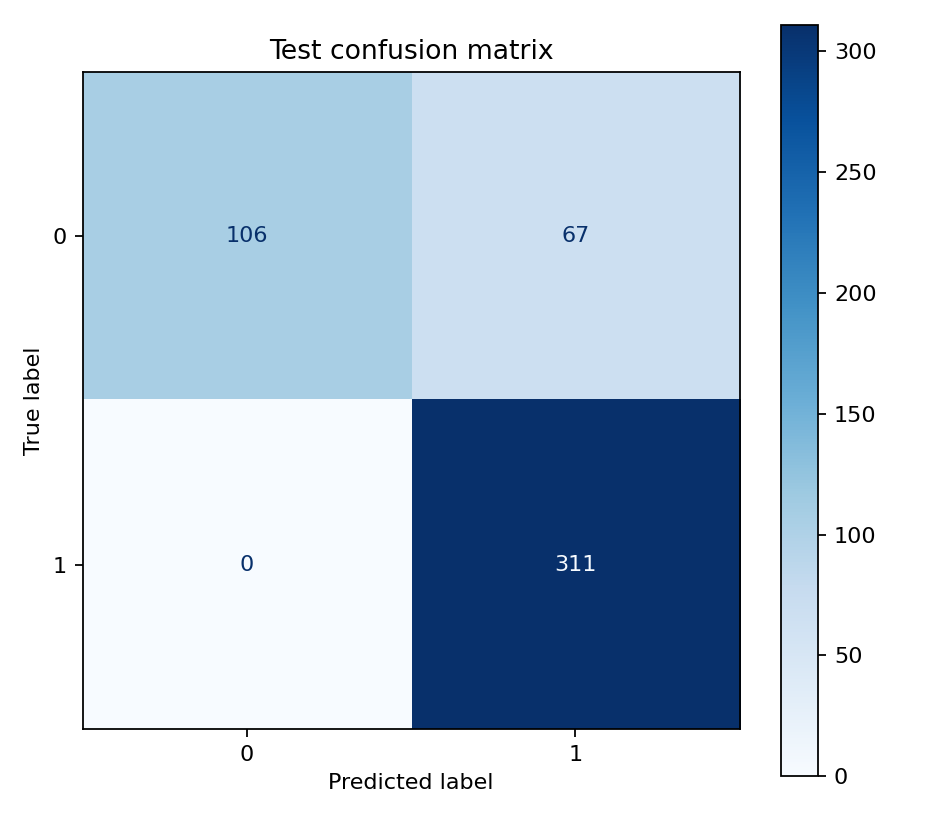
\includegraphics[width=\linewidth,height=0.60\textheight,keepaspectratio]{xjtu_gru_early_confusion_matrix.png}
      \smallcap{XJTU-SY GRU EarlyFault 混淆矩阵}
    \end{column}
    \begin{column}{0.48\textwidth}
      \centering
      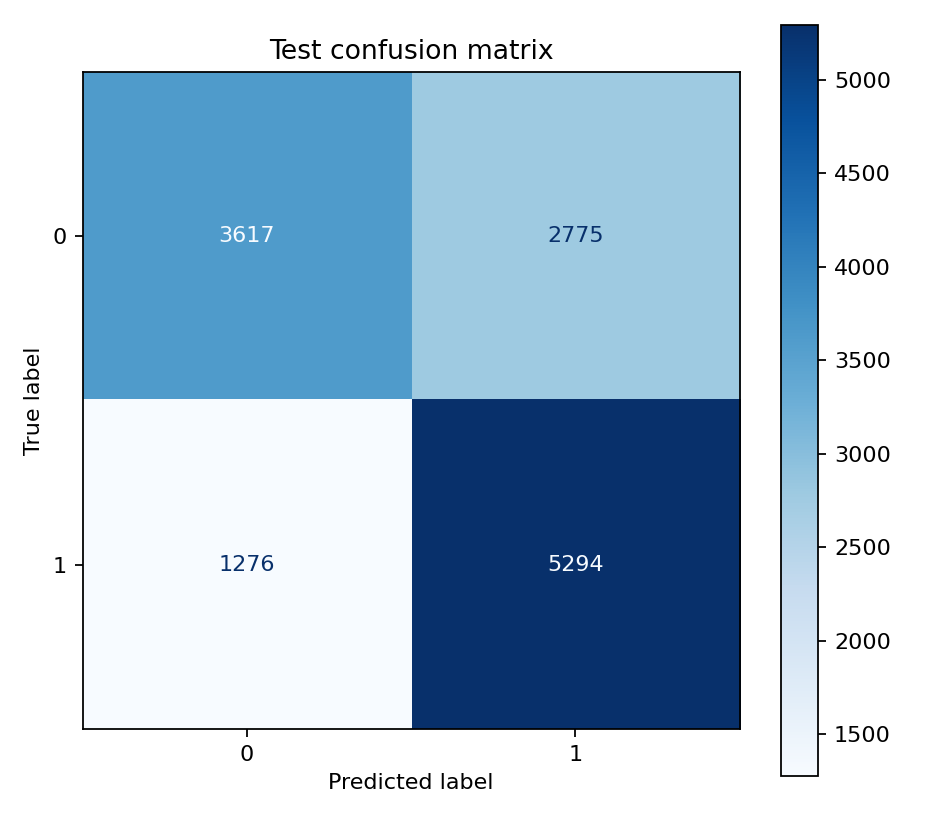
\includegraphics[width=\linewidth,height=0.60\textheight,keepaspectratio]{phm_gru_early_confusion_matrix.png}
      \smallcap{PHM2012 GRU EarlyFault 混淆矩阵}
    \end{column}
  \end{columns}

  \takeaway{EarlyFault 边界更粗，更适合表达是否进入预警阶段。}
\end{frame}

\section{复现与演示}

\begin{frame}[t]{论文复现实验：与已有方法参照}
  \begin{columns}[T,onlytextwidth]
    \begin{column}{0.48\textwidth}
      \begin{block}{PHM2012 RUL}
        \begin{itemize}
          \item CAM-LSTM 复现模型
          \item test RMSE = 0.146737
          \item MAE = 0.105007，R2 = 0.733183
        \end{itemize}
      \end{block}
      \centering
      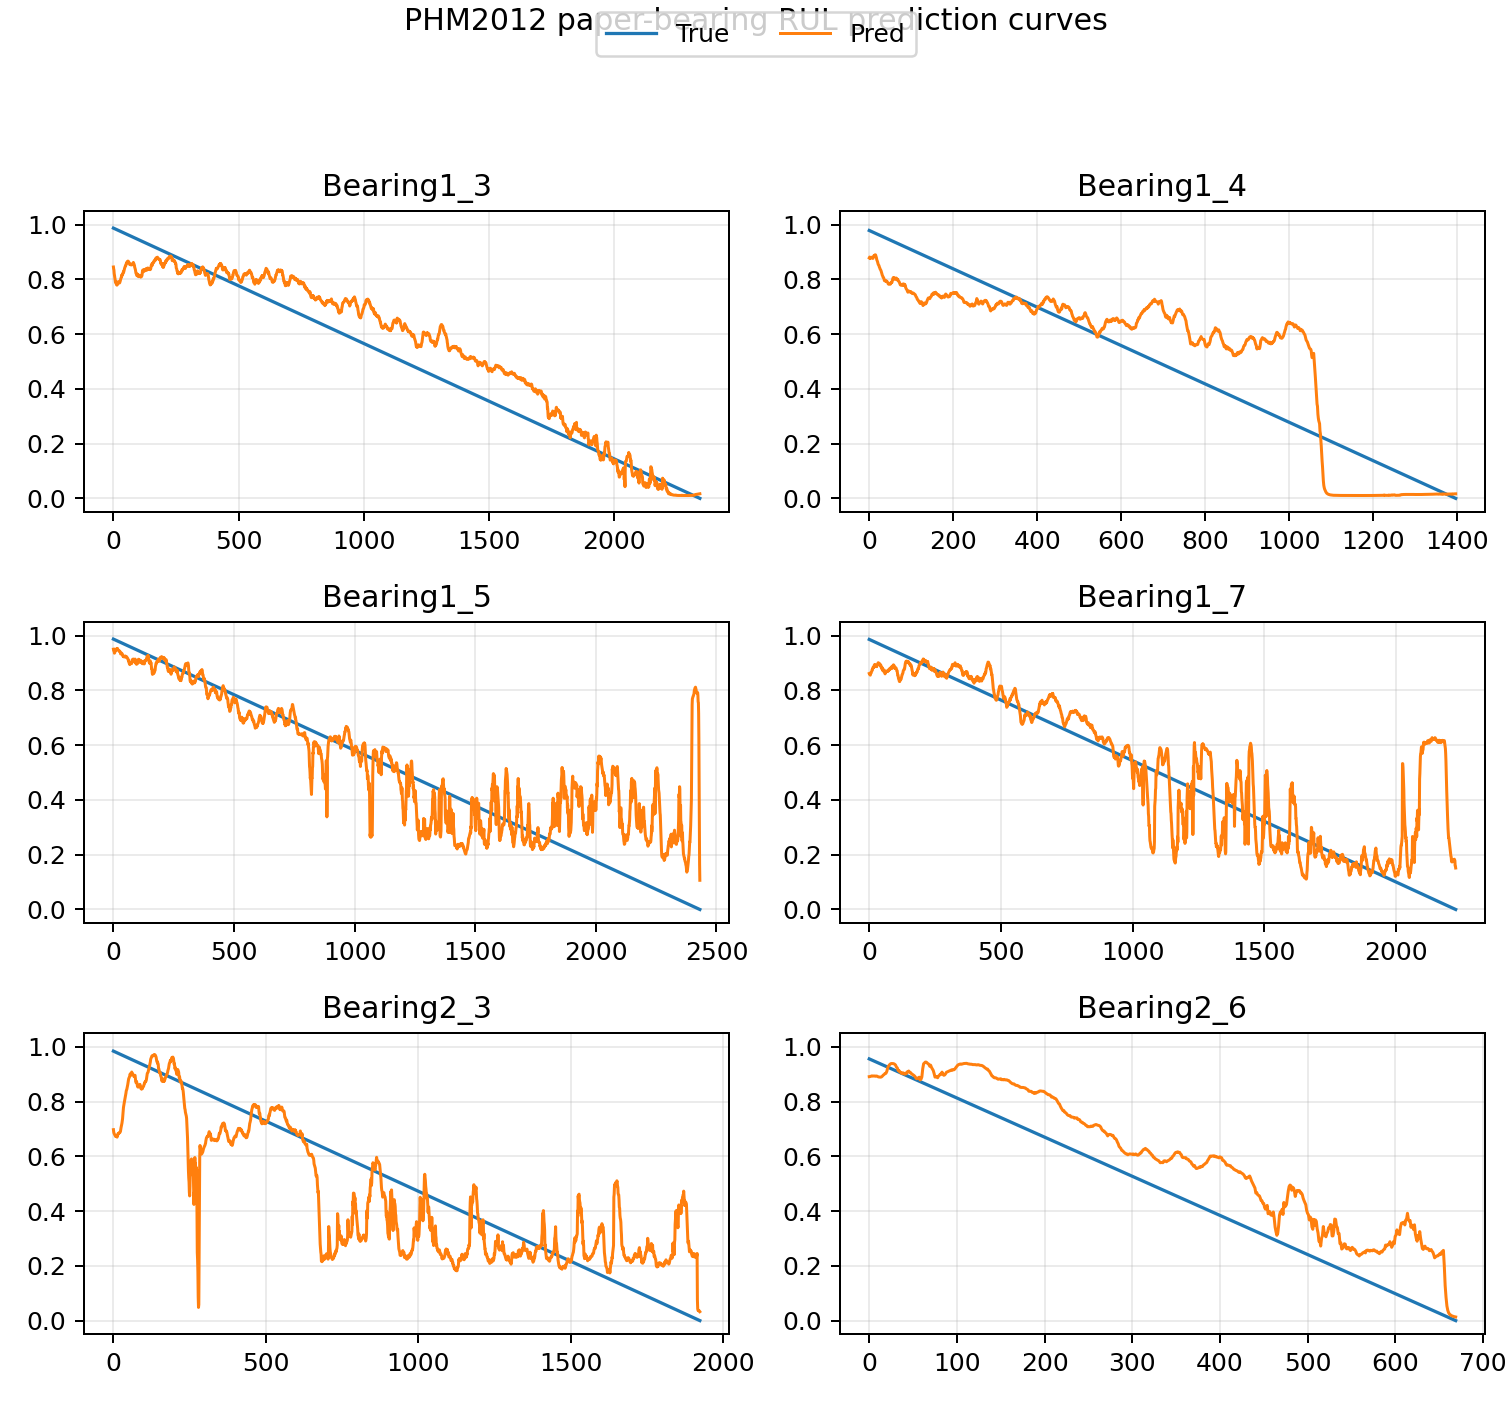
\includegraphics[width=\linewidth,height=0.33\textheight,keepaspectratio]{repro_phm_rul_prediction_by_bearing.png}
    \end{column}
    \begin{column}{0.48\textwidth}
      \begin{block}{XJTU-SY 故障诊断}
        \begin{itemize}
          \item 故障诊断复现模型
          \item test Accuracy = 0.997072
          \item WeightedF1 = 0.997072
        \end{itemize}
      \end{block}
      \centering
      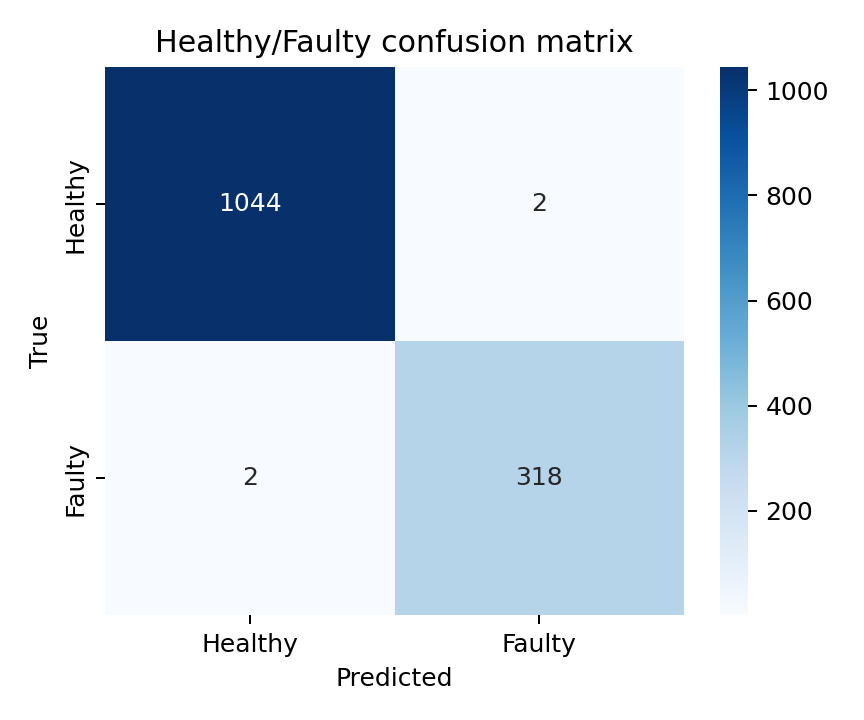
\includegraphics[width=\linewidth,height=0.33\textheight,keepaspectratio]{repro_xjtu_fault_confusion_matrix.png}
    \end{column}
  \end{columns}

  \vspace{0.25em}
  \scriptsize
  论文链接：
  \href{https://doi.org/10.3390/s25020554}{CBAM-CNN-LSTM RUL}
  \quad
  \href{https://doi.org/10.36001/IJPHM.2025.v16i1.4254}{Deep Learning Fault Diagnosis and Prognosis}

  \takeaway{复现实验验证论文方法复现能力，不替代本文三任务框架。}
\end{frame}

\begin{frame}[t]{现场命令演示}
  \begin{columns}[T,onlytextwidth]
    \begin{column}{0.54\textwidth}
      \begin{block}{演示目标}
        \begin{itemize}
          \item 读取 PHM2012 原始轴承数据
          \item 构造 manual\_basic 特征和三任务标签
          \item 运行 EarlyFault 二分类短训练
          \item 展示完整 CLI 训练链路
        \end{itemize}
      \end{block}
    \end{column}
    \begin{column}{0.43\textwidth}
      \begin{block}{重点观察}
        \begin{itemize}
          \item split 是否按官方语义加载
          \item label 是否包含 \code{early\_fault}
          \item sequence 是否不跨轴承
          \item metrics/report 是否正常生成
        \end{itemize}
      \end{block}
    \end{column}
  \end{columns}

  \vspace{0.6em}
  \begin{beamercolorbox}[wd=\linewidth,rounded=true,sep=0.65em]{block body}
    {\scriptsize\ttfamily
    uv run bp --config-name smoke mode=train dataset=phm2012 split=phm2012\_official\\
    feature=manual\_basic label=degradation\_three\_tasks task=early\_fault\_sequence\\
    model=gru trainer=base run.name=demo\_phm\_early\_fault\_gru\_5ep\\
    dataset.root=data/loader\_roots/phm2012 project.artifact\_root=artifacts/live\_demo\\
    task.cache\_dir=artifacts/live\_demo/cache\_phm\_early\_fault\\
    trainer.max\_epochs=5 trainer.batch\_size=256 trainer.console\_log.enabled=true}
  \end{beamercolorbox}
\end{frame}

\section{总结}

\begin{frame}[t]{不足与后续工作}
  \begin{columns}[T,onlytextwidth]
    \begin{column}{0.50\textwidth}
      \begin{block}{当前不足}
        \begin{itemize}
          \item RUL 泛化仍是主要难点
          \item HealthState / EarlyFault 是退化伪标签
          \item 物理故障频率特征尚未充分加入
          \item 尚未做完整超参数搜索
        \end{itemize}
      \end{block}
    \end{column}
    \begin{column}{0.47\textwidth}
      \begin{block}{未来方向}
        \begin{itemize}
          \item 加入 BPFO / BPFI / BSF / FTF 特征
          \item 尝试更强时序模型
          \item 多任务联合学习
          \item 跨工况训练与不确定性估计
        \end{itemize}
      \end{block}
    \end{column}
  \end{columns}
\end{frame}

\begin{frame}[t]{成员任务分配}
  \begin{table}
    \scriptsize
    \begin{tabularx}{\linewidth}{lcY}
      \toprule
      成员 & 贡献比例 & 主要工作 \\
      \midrule
      周逸进 & 25\% & 项目整合与论文复现：统一实验流程、GRU 序列模型、论文复现实验、结果整理与答辩材料组织。 \\
      朱德豪 & 25\% & 训练与评估：Trainer/Evaluator、训练配置、指标记录、对照实验运行与结果复核。 \\
      蔡祎珏 & 25\% & 数据与标签：XJTU-SY/PHM2012 数据加载、索引划分、RUL/HealthState/EarlyFault 标签构造。 \\
      邹扬 & 25\% & 特征与展示：manual\_basic 特征分析、可视化图表、展示材料整理、测试与交付检查。 \\
      \bottomrule
    \end{tabularx}
  \end{table}
\end{frame}

\begin{frame}[t]{总结}
  \begin{columns}[T,onlytextwidth]
    \begin{column}{0.58\textwidth}
      \begin{block}{完成内容}
        \begin{itemize}
          \item 完成 XJTU-SY 与 PHM2012 三任务数据链路
          \item 完成特征分析、标签构造和训练评估闭环
          \item 完成 GRU 序列模型实验结果与对照模型实验
          \item 完成论文复现实验和现场命令演示准备
        \end{itemize}
      \end{block}
      \begin{block}{一句话结论}
        本项目形成了可复查、可展示、可继续扩展的轴承 PHM 实验框架。
      \end{block}
    \end{column}
    \begin{column}{0.38\textwidth}
      \centering
      
\includegraphics[width=0.42\linewidth]{ustc_logo.pdf}
      \vspace{1em}

      {\Huge\bfseries\color{phmblue}谢谢老师！}

      \vspace{0.6em}
      {\large 轴承预测性维护系统}
    \end{column}
  \end{columns}
\end{frame}

\end{document}
